\chapter{IMPLEMENTASI}
	Bab ini membahas implementasi sistem pemantauan perangkat jaringan secara rinci. Pembahasan dilakukan secara rinci untuk setiap komponen yang ada, yaitu: REST API, Publisher server, Pub/sub Server, Server aplikasi dan websocket, Database server dan Antarmuka.
    
    \section{Lingkungan Implementasi}
    	Lingkungan implementasi dan pengembangan dilakukan menggunakan virtualisasi Proxmox dengan spesifikasi \textit{Host} komputer adalah Intel(R) Core(TM) i3-2120 CPU @ 3.30GHz dengan memori 8 GB di Laboratorium Arsitektur dan Jaringan Komputer, Teknik Informatika ITS. Perangkat lunak yang digunakan dalam pengembangan adalah sebagai berikut:
        \begin{itemize}
        \item Sistem Operasi Linux Ubuntu Server 16.04 LTS
        \item RabbitMQ 3.7.5-1
        \item MySQL Ver 15.1 Distrib 10.0.34-MariaDB
        \item Python 2.7
        \item Flask 0.12.2
        \item Node.js v6.11.4
        \item Nagios 4.3.4
        \item Express.js 4.16.3
        \end{itemize}
        
	\section{Implementasi REST API}
    	REST API digunakan untuk memudahkan aplikasi agar ringan dan mudah untuk dikembangkan. pada tugas akhir ini, REST API memiliki fungsi utama untuk menyimpan data user yang berlangganan pada perangkat jaringan atau berlangganan OID (Informasi didalam perangkat jaringan). REST API dibangun dengan framework Python yaitu Flask dan dilengkapi ORM (Object-relational mapping) Database yaitu Peewee.
        \subsection{Pemasangan Python Flask dan Peewee}
        	Pemasangan \texttt{Python Flask} dapat dilakukan dengan mudah, cukup dengan memasangnya dengan manajer paket yang dimiliki oleh \texttt{Python} yaitu \texttt{Pip}. Setelah \texttt{Flask} berhasil terpasang, selanjutnya adalah tahap pemasangan ORM \texttt{Peewee}. \texttt{Peewee} adalah Object-relational Mapping dimana fungsi utamanya adalah memudahkan pengembang agar dapat menyambungkan aplikasi dengan database dan melakukan query dengan mudah. pemasangan ORM Peewee dapat dilakukan dengan cara mengambil berkas instalasinya pada git \url{https://github.com/coleifer/peewee.git} dan pasang Peewee sesuai dengan instruksi yang tertera pada situs git tersebut.
        	
        \subsection{Implementasi Endpoint pada REST API }
        	REST API diakses menggunakan protokol HTTP. Penamaan dan struktur URL yang konsisten akan menghasilkan API yang baik dan mudah untuk dimengerti developer. URL API biasa disebut endpoint dalam pemanggilannya.
        	
        	Pada sistem ini terdapat beberapa endpoint, beberapa endpoint dibagi menjadi beberapa endpoint sesuai dengan perintah yang diajalankannya. misal: create, read, delete, update dan lain-lain.
        	
        	Berikut ini adalah endpoint yang dibuat dalam sistem ini:
        	
        	\begin{longtable}{|p{0.05\textwidth}|p{0.40\textwidth}|p{0.13\textwidth}|p{0.25\textwidth}|} % L = Rata kiri untuk setiap kolom, | = garis batas vertikal.
        		
        		% Kepala tabel, berulang di setiap halaman
        		\caption{Daftar Endpoint pada REST API} \label{tabelEndpointRESTAPI} \\
        		\hline
        		\textbf{No} & \textbf{Endpoint (Route)} & \textbf{Metode} & \textbf{Aksi} \\ \hline
        		\endhead
        		\endfoot
        		\endlastfoot
        		1 & /register & POST & Membuat data baru pada tabel user di database \\ \hline
        		2 & /login & POST & Mengambil data pada tabel user dan mencocokkannya dengan JSON yang dikirimkan lewat body. setelah data username dan password cocok, lalu dibuatkan sebuah token JWT. \\ \hline
        		3 & /logout & POST & Memasukkan token JWT yang terdaftar pada server kedalam daftar hitam agar token tidak dapat digunakan lagi. \\ \hline
        		4 & /users & GET & Menampilkan seluruh data user yang terdaftar pada sistem \\ \hline
        		5 & /users/\textless{}string:username\textgreater{} & GET & Menampilkan data user berdasarkan username yang tertulis pada URL \\ \hline
        		6 & /devices/create & POST & Membuat data baru pada tabel devices di database \\ \hline
        		7 & /devices/edit/\textless{}string:id\textgreater{} & PUT & Mengubah data pada tabel devices di database yang ID nya sama dengan ID yang ada pada URL. \\ \hline
        		8 & /devices/delete & DELETE & Menghapus data pada tabel devices di database yang ID nya tertulis pada body yang bertipe JSON. \\ \hline
        		9 & /devices & GET & Menampilkan seluruh data perangkat yang terdaftar pada sistem \\ \hline
        		10 & /devices/\textless{}string:id\textgreater{} & GET & Menampilkan data user berdasarkan username yang tertulis pada URL \\ \hline
        		11 & /oid/create & POST & Membuat data baru pada tabel oid \\ \hline
        		12 & /oid/edit & POST & Mengubah data pada tabel oid di database yang ID nya tertulis pada body yang bertipe JSON. \\ \hline
        		13 & /oid/delete & POST & Menghapus data pada tabel oid di database yang ID nya tertulis pada body yang bertipe JSON. \\ \hline
        		14 & /subscribe/devices & POST & Membuat data baru pada tabel subscribe \\ \hline
        		15 & /unsubscribe/devices & POST & Menghapus data pada tabel subscribe di database yang ID nya tertulis pada body yang bertipe JSON. \\ \hline
        		16 & /subscribe/oid & POST & Membuat data baru pada tabel subscribe\_oid \\ \hline
        		17 & /unsubscribe/oid & POST & Menghapus data pada tabel subscribe\_oid di database yang ID nya tertulis pada body yang bertipe JSON. \\ \hline	
        	\end{longtable}
        	
    
    \section{Implementasi Publisher Server}
    	Publisher server merupakan server yang berfungsi untuk mengambil data pada perangkat jaringan secara berkala dan mengirimkannya menuju pub/sub server. publisher server menggunakan plugin \texttt{check\_snmp} bawaan program Nagios, Sehingga untuk melakukan pengambilan data, kita perlu memasang nagios pada server.
    	
    	setelah data berhasil dikumpulkan, data yang diambil pada tiap perangkat dikirimkan menuju pub/pub server melalui thread yang berbeda. proses ini dinamakan \texttt{multithreading}.
    		\subsection{Pemasangan Nagios Sebagai Pemantau dan Pengumpul Data Perangkat}
    			Pemasangan \texttt{Nagios} dapat dilakukan dengan beberapa cara, namun cara yang dipakai pada kasus ini adalah memasang \texttt{Nagios} langsung dari sumbernya untuk mendapatkan fitur terbaru, pembaharuan keamanan, dan pembetulan bug.
    			
    			Berikut ini adalah sumber untuk mendapatkan nagios yang siap untuk dipasang: \url{https://assets.nagios.com/downloads/nagioscore/releases/nagios-4.3.4.tar.gz}
    			
    			\texttt{Nagios} perlu beberapa perintah khusus yang hanyak bisa dilakukan oleh user yang bernama "nagios" maka dari itu diperlukan user pada server yang bernama "nagios" dengan nama group "nagcmd". Selain user, \texttt{Nagios} juga perlu beberapa paket yang harus terpasang sebelum memasang nagios itu sendiri. Beberapa paket diantaranya adalah: \texttt{build-essential, libgd2-xpm-dev, openssl, libssl-dev, unzip}
    			
    			Setelah \texttt{Nagios} terpasang, direktori kerja dari Nagios dapat dilihat pada direktori \texttt{/usr/local/nagios}

			\subsection{Pengumpulan Data dan Pembuatan Script Pengiriman}
				Untuk mengumpulkan data perangkat jaringan, dibutuhkan plugin bawaan nagios yang bernama \texttt{check\_snmp}. plugin tersebut berada pada direktori \texttt{/usr/local/nagios/libexec} untuk menjalankan plugin tersebut dibutuhkan dua parameter, yaitu: alamat dari perangkat jaringan yang ingin dipantau dan OID dari data yang ingin didapatkan dari perangkat.
				perintah yang dijalankan untuk mendapatkan data pada perangkat jaringan lewat protokol SNMP adalah seeprti yang tertulis pada kode sumber 
				
\begin{lstlisting}[frame=single,breaklines,caption={Perintah Mengumpulkan Data Perangkat dengan SNMP},label=snmpcommand, captionpos=b]
$ /usr/local/nagios/check_snmp -H <alamat_perangkat> -o <oid_perangkat>
\end{lstlisting}
    			
    			Setelah data dapat dikumpulkan, sebuah script diperlukan untuk mengirim data tersebut menuju pub/sub server yang didukung boleh RabbitMQ sebagai Message Broker.
    			
    			Sebuah library bernama \texttt{pika} dibutuhkan untuk mengirim data tersebut ke pub/sub server. tiap perangkat yang dikumpulkan datanya dan dikirimkan ke pub/sub server, diproses didalam sebuah thread yang berbeda. oleh karena itu inisiasi database dibutuhkan pada awal script untuk menggetahui ada berapa perangkat yang terdaftar pada sistem.
    			
    			pertama-tama, masukkan library yang dibutuhkan untuk pembuatan script (termasuk pika), lalu dilanjutkan dengan potongan kode untuk menginisiasi database. Pseudocode untuk inisasi kelas database dapat dilihat pada kode sumber \ref{pseudo:dbclass}
    			
\begin{lstlisting}[frame=single,breaklines,caption={Pseudocode inisiasi Kelas Database},label=pseudo:dbclass, captionpos=b, language=json]
class BaseModel(Model):
class Meta:
database = database

class Users(BaseModel):
id = UUIDField(primary_key=True)
name = CharField()
username = CharField(unique=True)
password = CharField()
email = CharField()
role = CharField()

class Devices(BaseModel):
id = UUIDField(primary_key=True)
name = CharField()
type = CharField()
location = CharField()
address = CharField()

class Oid(BaseModel):
id = UUIDField(primary_key=True)
oid = CharField()
oidname = CharField()
devices_id = ForeignKeyField(Devices, on_delete='CASCADE')

class Subscribe(BaseModel):
users_id = ForeignKeyField(Users, on_delete='CASCADE')
devices_id = ForeignKeyField(Devices, on_delete='CASCADE')
\end{lstlisting}
    			
    			Setelah itu buat fungsi sebagai target menjalankan thread, nantinya tiap thread akan mengeksekusi kode yang ada didalam fungsi tersebut. didalam fungsi tersebut meliputi pegumpulan data dengan \texttt{check\_snmp}. Data perangkat jaringan yang dikumpulkan dengan \texttt{check\_snmp} dimasukkan kedalam sebuah \texttt{python dictionary} yang nantinya dictionary tersebut akan dikirimkan menuju pub/sub server. Pseudocode fungsi tersebut dapat dilihat pada kode sumber \ref{pseudo:threadtarget}
    			
\begin{lstlisting}[frame=single,breaklines,caption={Pseudocode Target \textit{Thread} Untuk Mengambil Data Perangkat},label=pseudo:threadtarget, captionpos=b, language=json]
rabbitMq(exchange, address):
	try:
		add getOidData() into array of dictionary
	except:
		add NULL into array of dictionary
	
	try:
		add getSnmpDeviceData() into JSON
	except:
		add Error Message into JSON		
\end{lstlisting}
    			
    			Untuk mengirimkan data menuju pub/sub server diperlukan library pika yang akan membuat koneksi dengan RabbitMQ yang berada di pub/sub server. Pseudocode untuk mengirimkan data tersebut dapat dilihat pada kode sumber \ref{pseudo:pika}
    			
\begin{lstlisting}[frame=single,breaklines,caption={Pseudocode Pengiriman Data Dengan Pika},label=pseudo:pika, captionpos=b, language=json]
pika.openConnection()
if exchange does not exist:
	createExchage()
	if queue does not exist:
		createQueue()
		bindExchangetoQueue()
	else:
		bindExchangetoQueue()
else:
	pass
sendMessage()
\end{lstlisting}
    			
				Setelah seluruh fungsi selesai dibuat, langkah terakhir adalah membuat thread agar tiap thread nantinya akan mejalankan fungsi yang telah dibuat dan menjalankannya secara berkala. Pseudocode untuk membuat thread dapat dilihat pada kode sumber \ref{pseudo:runthread}
				
\begin{lstlisting}[frame=single,breaklines,caption={Pseudocode Menjalankan Thread},label=pseudo:runthread, captionpos=b, language=json]
Thread
while true:
	getDeviceId() as exchangename
	getDeviceAddress as deviceaddress
	thread(target=rabbitmq(), argument=(exchangename, deviceaddress))
	sleep(2)

\end{lstlisting}

    \section{Implementasi Pub/Sub Server}
    	Pada pub/sub server, dipasang aplikasi message broker \texttt{RabbitMQ}. pada kasus ini \texttt{RabbitMQ} menerima seluruh data yang dikirmkan oleh publisher. Setelah itu, \texttt{RabbitMQ} menyimpannya dan menunggu hingga ada consumer yang meminta data pada \texttt{RabbitMQ}. kriteria data yang dikirimkan harus dispesifikkan sesuai dengan apa yang diminta oleh consumer.
    	
    	Pemasangan aplikasi \texttt{RabbitMQ} membutuhkan bahasa pemrograman \texttt{erlang}. untuk itu sebelum memasang \texttt{RabbitMQ}, harus terlebih dahulu memasang \texttt{erlang} pada sistem. Selain \texttt{erlang}, beberapa paket juga harus terpasang pada sistem, beberapa diantaranya adalah: \texttt{init-system-helpers, socat, adduser, logrotate}
    	
    	Setelah \texttt{RabbitMQ} server terpasang, selanjutnya dibutuhkan sebuah web admin untuk \texttt{RabbitMQ} agar mudah untuk melakukan manajemen data, user dan lain-lain pada web admin tersebut. \texttt{RabbitMQ} sudah menyediakan \textit{plugin} agar web admin dapat langsung digunakan. hanya dengan menjalankan perintah untuk mengaktifkan web admin dengan \texttt{rabbitmqctl}
    
    \section{Implementasi Consumer pada Server Aplikasi dan Websocket}
		Pada kasus ini, terdapat consumer yang diimplementasikan pada websocket. Websocket ini bertugas untuk meminta data pada pub/sub server yang telah dipasang \texttt{RabbitMQ}. Websocket ini disambungkan dengan suatu \textit{endpoint} pada server aplikasi, sehingga ketika \textit{client} mengakses endpoint pada aplikasi tersebut, javascript pada halaman tersebut akan menyambungkan halaman pada server websocket yang berada pada alamat dan port tertentu.
		
		Server websocket dibangun dengan menggunakan \texttt{node.js} dengan beberapa tambahan library. library yang digunakan pada websocket ini diataranya adalah: \texttt{Express.js} yang berperan sebagai kerangka kerja untuk membuat web dengan \texttt{node.js}, \texttt{http} untuk membuat webserver sederhana dengan \texttt{node.js}, \texttt{socket.io} unutk membuat komunikasi antara server dengan client menggunakan protokol websocket, dan \texttt{amqplib} untuk berkomunikasi dengan pub/sub server yang telah depasang \texttt{RabbitMQ}.
		
		implementasi inisiasi koneksi websocket dengan client dan pub/sub server dapat dilihat pada pseudocode yang terdapat pada kode sumber \ref{pseudo:initwebsocket}
		
\begin{lstlisting}[frame=single,breaklines,caption={Pseudocode Inisiasi Komunikasi Websokcet dengan Client dan Pub/Sub Server}, label=pseudo:initwebsocket, captionpos=b, language=json]
connectToRabbitMQServer()
createWebSocketConnection()
if websocketConnected():
	sendToClient('Connected')
else if websocketDisconnected():
	sendToClient('Disconnected') 
\end{lstlisting}

		Pada javascript yang terdapat pada client terdapat fungsi untuk menangkap pesan dari server bahwa websocket terlah berhasil tersambung. bersamaan saat websocket berhasil tersambung, \textit{client} mengirimkan seluruh id pada tabel \textit{devices} yang telah dilangggani oleh pengguna yang aktif untuk dijadikan nama pada exchange dan uuid versi 4 yang baru dibuat untuk memberi nama pada \textit{queue}.
		Pseudocode untuk fungsi tersebut dapat dilihat pada kode sumber \ref{pseudo:clientconnected}
		
\begin{lstlisting}[frame=single,breaklines,caption={Pseudocode Aktivitas Client Saat Terkoneksi dengan Websocket},label=pseudo:clientconnected, captionpos=b, language=json]
deviceID = getSubscribedDeviceIDbyUser()
pushDeviceIDToArray()
sendtoServer(deviceIDArray, uuid4())
\end{lstlisting}

		Setelah client mengirimkan id tiap perangkat dari tabel \textit{devices} untuk penamaan \textit{exchange} dan uuid versi 4 baru untuk penamaan queue, selanjutnya server akan memproses data tersebut untuk pembuatan queue dan exchange agar data pada pub/sub server dapat disalurkan lewat exchange dan queue tersebut. pseudocode aktivitas websocket server saat pembuatan queue dan exchange lalu menyalurkan data pada client dapat dilihat pada kode sumber \ref{pseudo:websocketrabbit}
		
\begin{lstlisting}[frame=single,breaklines,caption={Pseudocode Aktivitas Websocket Saat Pembuatan Queue dan Exchange Untuk Penyaluran Data ke Client},label=pseudo:websocketrabbit, captionpos=b, language=json]
if exchange does not exist:
	createExchage()
	if queue does not exist:
		createQueue()
		bindExchangetoQueue()
	else:
		bindExchangetoQueue()
else:
	pass

listenMessageFromRabbitMQServer()
sendMessageToClient()
\end{lstlisting}
		
    \section{Implementasi Database Server}
    	Sebagai media penyimpanan, sebuah database diperlukan untuk menyimpan data pengguna, perangkat, dan data berlangganan. Terdapat tiga tabel utama yang mewakili tiap entitas yang terlibat dalam sistem ini, yaitu: \texttt{users}, \texttt{devices}, dan \texttt{oid}. selain itu, terdapat dua table \texttt{many-to-many} untuk menyimpan data pengguna yang telah berlangganan kepada tiap perangkat dan pengguna yang berlangganan kepada tiap OID (untuk mengetahui informasi apa saja yang ada pada tiap perangkat. tiap OID memiliki informasi yang berbeda).
    	
    	Pada Tugas Akhir ini, sistem basis data yang digunakan adalah \texttt{Mysql Server} yang dimana \texttt{Mysql Server} termasuk kedalam RDBMS (\textit{Relational Database Management System}). Berikut adalah rincian dari tabel yang diimplementasikan. rincian tabel \texttt{users} dapat dilihat pada tabel \ref{tabeldbusers}
    	
    	\begin{longtable}{|p{0.05\textwidth}|p{0.20\textwidth}|p{0.22\textwidth}|p{0.35\textwidth}|} % L = Rata kiri untuk setiap kolom, | = garis batas vertikal.
    		
    		% Kepala tabel, berulang di setiap halaman
    		\caption{Rincian Tabel \texttt{users} pada Database} \label{tabeldbusers} \\
    		\hline
    		\textbf{No} & \textbf{Kolom} & \textbf{Tipe Data} & \textbf{Keterangan} \\ \hline
    		\endhead
    		\endfoot
    		\endlastfoot
    		1 & id & varchar(255) & Sebagai primary key pada tabel, nilai pada kolom ini berformat UUID versi 4 \\ \hline
    		2 & name & varchar(255) & Data yang berbentuk string. Digunakan untuk kelengkapan profil pengguna. \\ \hline
    		3 & username & varchar(255) & Data yang berbentuk string. Digunakan untuk keperluan autentikasi. \\ \hline
    		4 & password & varchar(255) & Data yang berbentuk string, implementasinya berupa hash. Digunakan untuk keperluan autentikasi. \\ \hline
    		5 & email & varchar(255) & Data yang berbentuk string. Digunakan untuk kelengkapan profil pengguna \\ \hline
    		6 & role & varchar(255) & Data yang berbentuk string. Digunakan untuk kelengkapan profil pengguna dan pembeda peran agar setiap user memiliki hak istimewa masing-masing. \\ \hline
    	\end{longtable}
    	
    	Terdapat juga tabel \texttt{devices} yang digunakan untuk menyimpan seluruh data perangkat. pada tabel ini terdapat lima kolom. rincian tabel \texttt{devices} dapat dilihat pada tabel \ref{tabeldbdevices}
    	
    	\begin{longtable}{|p{0.05\textwidth}|p{0.20\textwidth}|p{0.22\textwidth}|p{0.35\textwidth}|} % L = Rata kiri untuk setiap kolom, | = garis batas vertikal.
    		
    		% Kepala tabel, berulang di setiap halaman
    		\caption{Rincian Tabel \texttt{devices} pada Database} \label{tabeldbdevices} \\
    		\hline
    		\textbf{No} & \textbf{Kolom} & \textbf{Tipe Data} & \textbf{Keterangan} \\ \hline
    		\endhead
    		\endfoot
    		\endlastfoot
    		1 & id & varchar(255) & Sebagai primary key pada tabel, nilai pada kolom ini berformat UUID versi 4 \\ \hline
    		2 & name & varchar(255) & Data yang berbentuk string. Digunakan untuk kelengkapan profil dari perangkat jaringan. \\ \hline
    		3 & type & varchar(255) & Data yang berbentuk string. Digunakan untuk kelengkapan profil dari perangkat jaringan. \\ \hline
    		4 & location & varchar(255) & Data yang berbentuk string. Digunakan untuk kelengkapan profil dari perangkat jaringan. \\ \hline
    		5 & address & varchar(255) & Data yang berbentuk string, implementasinya barbentuk alamat IP dari tiap perangkat jaringan. Digunakan untuk mengkoleksi data pada publisher server. \\ \hline
    	\end{longtable}
    	
    	lalu terdapat juga tabel \texttt{OID} yang digunakan untuk menyimpan seluruh data informasi yang tersedia pada tiap perangkat. Pada tabel ini terdapat tiga kolom utama dan satu kolom \textit{foreign key} yang terhubung dengan tabel \texttt{devices}. Rincian tabel \texttt{OID} dapat dilihat pada tabel \ref{tabeldboid}
    	
    	\begin{longtable}{|p{0.05\textwidth}|p{0.20\textwidth}|p{0.22\textwidth}|p{0.35\textwidth}|} % L = Rata kiri untuk setiap kolom, | = garis batas vertikal.
    		
    		% Kepala tabel, berulang di setiap halaman
    		\caption{Rincian Tabel \texttt{OID} pada Database} \label{tabeldboid} \\
    		\hline
    		\textbf{No} & \textbf{Kolom} & \textbf{Tipe Data} & \textbf{Keterangan} \\ \hline
    		\endhead
    		\endfoot
    		\endlastfoot
    		1 & id & varchar(255) & Sebagai primary key pada tabel, nilai pada kolom ini berformat UUID versi 4 \\ \hline
    		2 & oid & varchar(255) & Data yang berbentuk string, implementasinya berbentuk OID (Object-Identifier). Digunakan mengkoleksi perangkat jaringan pada publisher server. \\ \hline
    		3 & oidname & varchar(255) & Data yang berbentuk string. Digunakan untuk kelengkapan profil dari perangkat jaringan. \\ \hline
    		4 & devices\_id & varchar(255) & Merupakan foreign key dari id pata tabel \texttt{devices}. Data ini berbentuk string, nilai pada kolom ini berformat UUID versi 4. \\ \hline
    	\end{longtable}
    
    	lalu terdapat juga tabel \texttt{subscribe} yang digunakan untuk menyimpan seluruh data pengguna (\textit{user}) yang berlangganan informasi pada tiap perangkat. Tabel ini bersifat \textit{many-to-many}, pada tabel ini terdapat dua kolom \textit{foreign key} yang terhubung dengan tabel \texttt{devices} dan \texttt{users}. Rincian tabel \texttt{subscribe} dapat dilihat pada tabel \ref{tabeldboid}
    
    	\begin{longtable}{|p{0.05\textwidth}|p{0.20\textwidth}|p{0.22\textwidth}|p{0.35\textwidth}|} % L = Rata kiri untuk setiap kolom, | = garis batas vertikal.
    		
    		% Kepala tabel, berulang di setiap halaman
    		\caption{Rincian Tabel \texttt{subscribe} pada Database} \label{tabeldbsubscribe} \\
    		\hline
    		\textbf{No} & \textbf{Kolom} & \textbf{Tipe Data} & \textbf{Keterangan} \\ \hline
    		\endhead
    		\endfoot
    		\endlastfoot
    		1 & users\_id & varchar(255) & Sebagai primary key pada tabel juga sebagai foreign key dari id pada tabel \texttt{users}, nilai pada kolom ini berformat UUID versi 4 \\ \hline
    		2 & devices\_id & varchar(255) & Sebagai primary key pada tabel juga sebagai foreign key dari id pada tabel \texttt{devices}, nilai pada kolom ini berformat UUID versi 4. \\ \hline
    	\end{longtable}
    	
    	terakhir, terdapat tabel \texttt{subscribeoid} yang digunakan untuk menyimpan seluruh data pengguna (\textit{user}) yang berlangganan informasi pada tiap perangkat. Tabel ini bersifat \textit{many-to-many}, pada tabel ini terdapat dua kolom \textit{foreign key} yang terhubung dengan tabel \texttt{OID} dan \texttt{users}. Rincian tabel \texttt{subscribe}oid dapat dilihat pada tabel \ref{tabeldbsubscribeoid}
    	
    	\begin{longtable}{|p{0.05\textwidth}|p{0.20\textwidth}|p{0.22\textwidth}|p{0.35\textwidth}|} % L = Rata kiri untuk setiap kolom, | = garis batas vertikal.
    		
    		% Kepala tabel, berulang di setiap halaman
    		\caption{Rincian Tabel \texttt{subscribeoid} pada Database} \label{tabeldbsubscribeoid} \\
    		\hline
    		\textbf{No} & \textbf{Kolom} & \textbf{Tipe Data} & \textbf{Keterangan} \\ \hline
    		\endhead
    		\endfoot
    		\endlastfoot
    		1 & users\_id & varchar(255) & Sebagai primary key pada tabel juga sebagai foreign key dari id pada tabel \texttt{users}, nilai pada kolom ini berformat UUID versi 4 \\ \hline
    		2 & oid\_id & varchar(255) & Sebagai primary key pada tabel juga sebagai foreign key dari id pada tabel \texttt{oid}, nilai pada kolom ini berformat UUID versi 4. \\ \hline
    	\end{longtable} 

    \section{Implementasi Antarmuka}
    	Antarmuka sistem dibangun dengan menggunakan \texttt{Bootstrap4} dan \texttt{Jquery} pada \textit{frontend} dan kerangka kerja \texttt{Flask} pada \textit{backendn}nya. Antarmuka yang utama digunakan pada tugas akhir ini digunakan untuk mempermudah pengelolaan data perangkat dan halaman pemantauan perangkat jaringan. Antarmuka yang diimplementasikan pada tugas akhir ini adalah sebagai berikut:
    	\begin{itemize}
    		\item Menampilkan seluruh data perangkat yang terdaftar pada sistem
    		\item Menampilkan rincian data perangkat jaringan yang terdaftarpada sistem
    		\item Menampilkan data yang ingin dipantau pengguna pada sistem
    	\end{itemize}
		\subsection{Menampilkan seluruh data perangkat yang terdaftar pada sistem}
        	Halaman ini berfungsi untuk menampilkan seluruh data yang terdaftar pada sistem. Seluruh data disajikan dalam bentuk tabel data yang dibangun dengan menggunakan bootstrap4, sehingga memungkinkan pengguna untuk mencari dan mengurutkan dapat pada tabel. Antarmuka daftar perangkat pada sistem ditunjukkan pada Gambar \ref{antarmuka:daftarperangkat}.
			\begin{figure}[H]
				\centering
				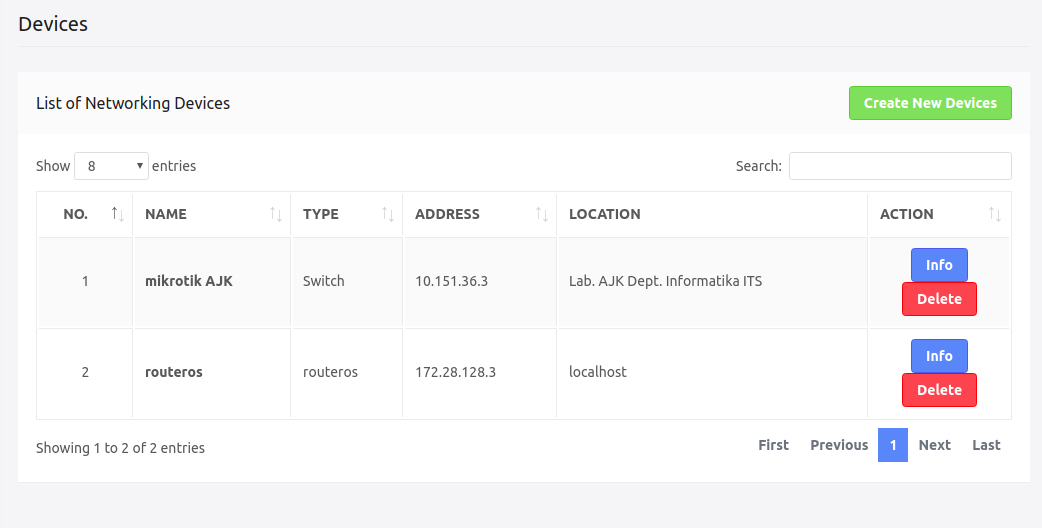
\includegraphics[width=11.2cm]{Images/C-4/antarmukadaftarperangkat.png}
				\caption{Dasbor Daftar Aplikasi}
				\label{antarmuka:daftarperangkat}
			\end{figure}
            
         \subsection{Menampilkan rincian data perangkat jaringan yang terdaftarpada sistem}
         	Halaman ini berfungsi untuk menunjukkan informasi tiap perangkat. Informasi yang disajikan meliputi informasi umum tiap perangkat (nama perangkat, tipe perangkat, alamat perangkat dan lokasi perangkat), daftar pengguna yang berlangganan ke perangkat tersebut, dan daftar OID (informasi keadaan perangkat) yang tersedia pada perangkat tersebut.
         	
         	Pada halaman ini pengguna dapat berlangganan kepada perangkat dengan menekan tombol subscribe pada kolom "\textit{Subscriber}". setelah berhasil berlangganan kepada perangkat, sistem akan menampilkan tombol "\textit{subscribe}" pada kolom OID, dimana tombol tersebut berfungsi untuk memilih informasi apa saja yang ingin didapatkan oleh pengguna. Antarmuka informasi ditunjukkan pada Gambar \ref{antarmuka:rincianperangkat}.
         	\begin{figure}[H]
         		\centering
         		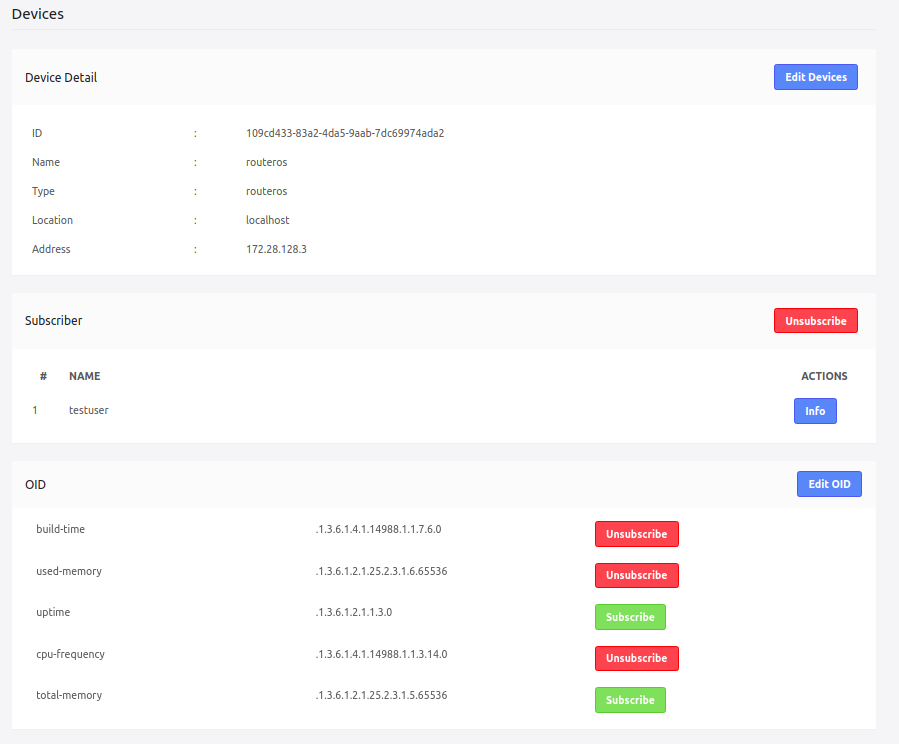
\includegraphics[width=11.2cm]{Images/C-4/antarmukarincianperangkat.png}
         		\caption{Dasbor Informasi Aplikasi}
         		\label{antarmuka:rincianperangkat}
         	\end{figure}
            
         \subsection{Menampilkan data yang ingin dipantau pengguna pada sistem}
         	Pada halaman ini, pengguna dapat memantau atau melihat kondisi dari tiap perangkat yang telah dilanggani oleh tiap pengguna. Informasi yang disajikan pada halaman ini tergantung dari banyaknya informasi pada tiap perangkat yang dilanggani oleh pengguna. pada halaman ini juga, websocket bekerja. jika \textit{client} (\textit{browser}) terkoneksi dengan websocket, maka akan terdapat kotak berwarna hijau pada bagian atas halaman, sedangkan jika \textit{client} tidak terhubung dengan websocket maka kotak tersebut akan berwarna merah. Antarmuka halaman daftar \textit{container} ditunjukkan pada Gambar \ref{antarmuka:pantau}.
            \begin{figure}[H]
				\centering
				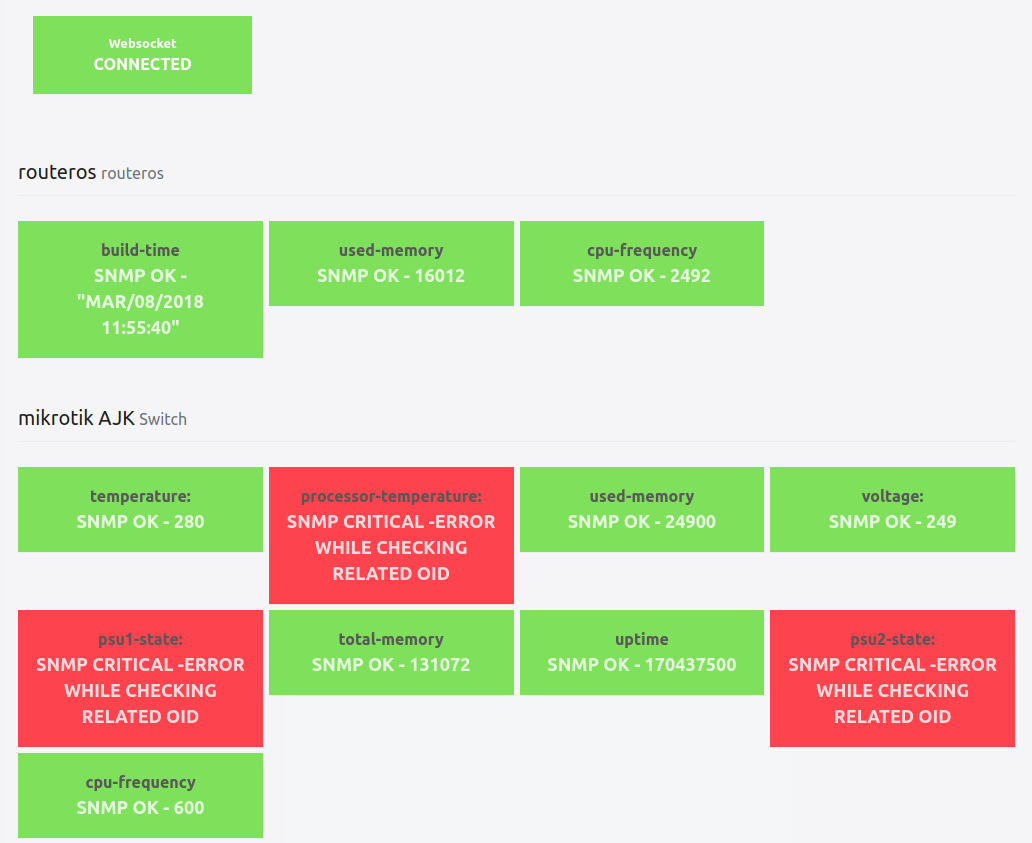
\includegraphics[width=11.2cm]{Images/C-4/antarmukapantau.png}
				\caption{Dasbor Daftar \textit{Container}}
				\label{antarmuka:pantau}
			\end{figure}